% qjrms4doc.tex V1.00, 30 July 2010


%\documentclass[times, doublespace]{qjrms4}
%\onecolumn
\documentclass[times]{qjrms4}
%\documentclass[dvips,12pt,twoside]{article}
\usepackage[dvips,colorlinks,bookmarksopen,bookmarksnumbered,citecolor=red,urlcolor=red]{hyperref}

\usepackage{natbib}
\setlength{\bibsep}{1pt}
\newcommand{\bibfont}{\footnotesize}

%\numberwithin{equation}{section}

\newcommand\BibTeX{{\rmfamily B\kern-.05em \textsc{i\kern-.025em b}\kern-.08em
T\kern-.1667em\lower.7ex\hbox{E}\kern-.125emX}}

\usepackage{moreverb}

\def\volumeyear{20??}
\def\volumenumber{00}

\begin{document}
\runningheads{R.~E.~Petrie et al}{Toy Model}

\title{A non-hydrostatic toy model for use in convective-scale data assimilation}%\footnotemark[2]}

\author{R.~E.~Petrie,\affil{a}\corrauth\
R.~N.~Bannister,\affil{a}, M.J.P.~Cullen\affil{b} }

\address{\affilnum{a} Department of Meteorology, University of Reading, UK
\\
\affilnum{b} UK Met Office, Fitzroy Road, Exeter}
%
\corraddr{Department of Meteorology, Earley Gate, Whiteknights Campus, University of Reading, Reading, RG6 6BB. E-mail: r.e.petrie@reading.ac.uk}

%%%%%%%%%%%%%%%%%%%%%%%%%%%%%%%%%%%%%%%%%%%%%%%%%%%%%%%%%%%%%%%%%%%%%%%%%%%%%%%%%%%%%%%%%%%%%%%%%%%%
\begin{abstract}
In developing methods for convective-scale data assimilation it is necessary to consider
non-hydrostatic and ageostrophic flow governed by the fully compressible Navier-Stokes equations. These equations describe a wide range of time-scales with complex nonlinear coupling. It is thus very helpful to consider simpler systems when developing new techniques. However, to be useful for this application, such systems need to permit 
large-scale hydrostatic and geostrophic balance while allowing small-scale imbalance. In particular, they need to
exhibit intermittent convective-like behaviour.  Existing highly idealized models are not sufficient
 for investigating these issues.  A simplified system of intermediate complexity derived from the Euler equations is therefore presented in this paper. In this system the separation of time scale is greatly reduced by changing the physical parameters. This allows acoustic modes to be treated explicitly. In addition, the nonlinear coupling induced by the equation of state is simplified. This means that the gravity and acoustic modes can be treated separately, while in the real system they are always coupled even at the level of a normal mode analysis. A vertical slice formulation is used which contains only dry dynamics. However, the necessary intermittent convective behaviour is generated by localised compressible effects.
This model provides an affordable and flexible framework within which some of the complex issues 
of convective-scale data assimilation can be investigated.
 
\end{abstract}
%%%%%%%%%%%%%%%%%%%%%%%%%%%%%%%%%%%%%%%%%%%%%%%%%%%%%%%%%%%%%%%%%%%%%%%%%%%%%%%%%%%%%%%%%%%%%%%%%%%%

\keywords{Convective-scale modelling; Non-hydrostatic model}

\maketitle

%\footnotetext[2]{Please ensure that you use the most up to date%
%class file,
%available from the QJRMS Home Page at\\
%\href{http://www.interscience.wiley.com/qj}{\texttt{http://www.interscience.wiley.com/qj}}%
%}

%%%%%%%%%%%%%%%%%%%%%%%%%%%%%%%%%%%%%%%%%%%%%%%%%%%%%%%%%%%%%%%%%%%%%%%%%%%%%%%%%%%%%%%%%%%%%%%%%%%%
%===================================================================================================
\section{Introduction}\label{intro} 

Advances in computer power have enabled Numerical Weather Prediction (NWP) models to 
operate at higher resolutions than has previously been possible.  
%
In 2009 the United Kingdom Meteorological Office (UK Met. Office) upgraded the 
resolution of its Unified Model (UM), \citep{davies_2005}, for the UK domain from $12 \rm{km}$ to $1.5 \rm {km}$,
\citep{dixon_2009}. 
%
Resolutions of this degree are expected to resolve the large and synoptic scale features well.
\cite{bryan_2003} find that models with resolutions of $100 \rm {m} $ are necessary 
to provide meaningful simulations of convection. 
%
Resolutions of $O(100\rm{m})$ are not yet affordable over the UK domain with current computer resources, though research experiments with the UM over smaller domains with  $200 \rm{m}$ resolution have shown marked benefit, ???citation to Lean needed. 
%
Models of this resolution are known as convective-scale models because they are capable of 
resolving some convection explicitly, thus do not require a convection parameterization scheme.  
%
For instance it is possible to explicitly represent smaller scale features, 
such as thunderstorms of $O(10 \rm{km})$ 
and Mesoscale Convective Systems (MCSs) of $O(10-100 \rm{km})$, though not resolve their 
internal structure (e.g. \cite{bryan_2003, clark_2005, lean_2008}).  
%
Convective-scale forecasting can facilitate more accurate and earlier indications of extreme or hazardous 
weather, e.g. severe convection \citep{lean_2008}, which is of clear benefit.  

As NWP moves towards the convective-scale so it is appropriate to examine the data 
assimilation scheme underpinning the forecast. 
The data assimilation process takes 
meteorological data from a variety of sources including satellites, radar, ground 
based weather stations and radiosondes and combines them with a previous forecast 
to produce an analysis (e.g. \cite{daley_1991}, \cite{kalnay}).  The NWP model 
is then integrated forward from the analysed state.
The data assimilation scheme that combines the observed data with the background state 
should provide an analysis that is physically, spatially and temporally 
consistent \citep{daley_1991}.  
The motivation for the development of this model is a detailed and technical investigation of
the convective-scale data assimilation problem though the utility of this model is not limited to 
this application.

Convective-scale data assimilation introduces new issues. The errors in the larger-scale flow are still present, but in addition there will be errors on the small scales resolved by the convective-scale model which will have a very different correlation structure. A pragmatic solution is to rely on a larger scale data assimilation to correct the large-scale errors, and thus allow convective-scale data asimilation to focus on small scales. The model introduced in this paper is intended to develop methods of assimilating the small-scale information. Detailed 
reviews of the issues are given by  \cite{dance_2004, lorenc_2007, park_2003, sun_2005}.  
The current Met Office operational large-scale data assimilation scheme enforces hydrostatic balance 
as a strong constraint and exploits geostrophy as a weak constraint in the covariance model 
\citep{lorenc_2000,bannister_2008_2}.  
The use of the hydrostatic balance relationship is valid for flows where the aspect ratio is much 
less than one (e.g. \citep{holton, vallis}. 
In regions of convection the aspect ratio increases and so hydrostatic balance may no longer be a good approximation.  
\cite{vetra_2012} demonstrated that hydrostatic balance breaks down in the UM when it is run
at $1.5 \rm {km}$ horizontal resolution.
In the mid and high latitudes the geostrophic assumption is accurate for large-scale flows where the Rossby number is small (e.g. \cite{holton}). 
At the convective-scale the Rossby number is not small and therefore the use of geostrophic balance  
is no longer appropriate. 
It is therefore important that these balances are relaxed in convective-scale data assimilation.

%A convective-scale forecast model tries to predict convective features which are 
%often coupled to the larger scale flow (e.g. from forcing due to frontal systems).  
%It is therefore arguable that both the large and small-scale information is dealt with 
%appropriately and simultaneously in the data assimilation process \citep{dixon_2009}.  
%The utility of high resolution data assimilation is to improve the analysis estimate for 
%the smaller scale features, while ensuring that information on the large-scale is 
%not lost at its expense \citep{baxter}.  

Operational systems have to resolve features at both the synoptic and the convective-scales, 
requiring a large number of grid points.  
Such systems are very expensive to run and are not ideal tools for research purposes. The wide range of time-scales means that semi-implicit integration schemes are required for efficiency, e.g. \citep{davies_2005}, and the nonlinear coupling between acoustic and gravity waves through the equation of state makes analysing the small-scale behaviour difficult, \citep{thuburn1}. This it would be useful to have a somewhat idealized model which describes a variety of regimes but without the extreme separation of time-scales and the nonlinear coupling between acoustic and gravity waves present in the real system. 
A simplified system which has these properties allows problems such as the convective-scale 
data assimilation problem to be explored in a practical but physically
realistic way.

The simplified system derived in this paper is intended to be run in vertical slice geometry, so that many fewer degrees of freedom are needed than in an operational three-dimensional system. The equations are modified so that the speed of acoustic and gravity waves can be controlled, and the large separations in time-scales reduced. The equation of state and pressure gradient terms are also modified so that the acoustic and gravity waves decouple. The modifications are designed so that energy is conserved, which is necessary for realistic long-time behaviour. No moisture is included, but instead localised regions where compressible effects dominate simulate the intermittent convective like behaviour which is characteristic of 
the real system.  
These simplifications permit large-scale balanced flows and sporadic small-scale non-hydrostatic 
flows (i.e. convection) to coexist within the framework of a simplified and practical model. 
This system is therefore a useful tool for investigating the convective-scale 
data assimilation problem. 

Section \ref{derivation} provides a derivation of the toy model equations which are analysed in 
terms a scale analysis and energy conservation properties. 
Section \ref{linanal} provides a linear analysis of the equations. Section \ref{behav} 
shows the results of an idealized integration which illustrates geostrophic adjustment
and demonstrates how the model can be used to simulate different types of flow regime and section 

??? A lot more needed here.
\ref{summ} provides a summary and some concluding remarks. Future work will exploit 
this model in testing different approaches to convective-scale data assimilation.

%===================================================================================================
\section{Derivation of the model equations}\label{derivation}

The model is derived from the standard compressible 3-dimensional Euler equations 
(\ref{mom_euler}) - (\ref{eqnstat_euler}). Derivations of these equations 
are well covered in the literature, see for example \cite{holton, pielke, vallis}.

%^^^^^^^^^^^^^^^^^^^^^^^^^^^^^^^^^^^^^^^^^^^^^^^^^^^^^^^^^^^^^^^^^^^^^^^^^^^^^^^^^^^^^^^^^^^^^^^^^^^
\begin{subequations} \label{euler_eqns}
\begin{align}
    \frac{\partial \mathbf u}{\partial t} + \mathbf u \cdot \nabla \mathbf u + 
    \frac{1}{\rho} \nabla p + g \mathbf k  + 2\Omega \times \mathbf u &=  0,  \label{mom_euler} \\
   \frac {\partial \rho}{\partial t}  +  \nabla \cdot  
   \left(\rho \mathbf u \right) &=  0 ,  \label{cont_euler}\\
   \frac{\partial \theta}{\partial t} +  \mathbf u  \cdot  
   \nabla \theta &= 0, \label{thermo_euler}\\
    p = \rho R \left( \frac {p}{p_{00}} \right)^{\kappa} \theta .  \label{eqnstat_euler}
\end{align}
\end{subequations}
%^^^^^^^^^^^^^^^^^^^^^^^^^^^^^^^^^^^^^^^^^^^^^^^^^^^^^^^^^^^^^^^^^^^^^^^^^^^^^^^^^^^^^^^^^^^^^^^^^^^

Equation (\ref{mom_euler}) are the momentum equations. The wind vector is $\mathbf u = (u, v, w)$ 
where the zonal component is $u$, the meridional component is $v$ and the vertical 
component is $w$. Pressure is $p$ and the acceleration due to gravity is $g$. 
The \textit{f-plane} assumption is made such that the Earth's angular momentum vector $2\Omega = f \mathbf k$ where $f$ 
is a constant and $\mathbf k$ is the unit vector in the vertical direction.
Equation (\ref{cont_euler}) is the compressible mass continuity equation where $\rho$ is the density.  
Equation (\ref{thermo_euler}) is the adiabatic thermodynamic equation where $\theta$ is potential 
temperature. Equation (\ref{eqnstat_euler}) is the equation of state for an ideal gas written in 
terms of potential temperature, $p_{00}$ is the $1000 \rm{ hPa}$ reference pressure, 
$\kappa = R/{c_p}$ is a constant, with $c_p$ the specific heat capacity at a constant pressure 
and $R$ the gas constant for dry air. 

From this set of equations we wish to construct a toy model that has large-scale geostrophically and
hydrostatically balanced flow, permits intermittent convective behaviour and is of practical use
for investigating issues that arise in the convective-scale data assimilation problem.


%--------------------------------------------------------------------------------------------------- 
\subsection{Modifications}

In order to derive a model with the properties outlined above 
the Euler equations (\ref{euler_eqns}) are modified in two stages. Firstly, a set of physically based approximations are made and secondly a set of 
toy model simplifications are made. The toy model simplifications do not attempt to replicate 
the real system, rather they are intended to retain desired physical characteristics of the real system
in the model while simplifying the numerical and computational implementation.
In order to simplify the system it will be assumed that the model is periodic in the zonal direction 
and homogeneous in the meridional direction (i.e. the variables are functions
of longitude and height only). 

%- - - - - - - - - - - - - - - - - - - - - - - - - - - - - - - - - - - - - - - - - - - - - - - - - -
\subsubsection{Physically based approximations}

The variables are decomposed such that they have a basic state and perturbation component
as in for example \citet{pielke}.
%^^^^^^^^^^^^^^^^^^^^^^^^^^^^^^^^^^^^^^^^^^^^^^^^^^^^^^^^^^^^^^^^^^^^^^^^^^^^^^^^^^^^^^^^^^^^^^^^^^^
   \begin{eqnarray} \label{basic_state}
     \Phi(x,z, t) &=& \Phi_0(z) + \Phi'(x,z, t), \label{e_def_vars} \\ 
     \theta(x,z, t) &=& \theta_{\rm R} + \theta_0(z) + \theta'(x,z, t), \label{e_def_theta}
   \end{eqnarray}
%^^^^^^^^^^^^^^^^^^^^^^^^^^^^^^^^^^^^^^^^^^^^^^^^^^^^^^^^^^^^^^^^^^^^^^^^^^^^^^^^^^^^^^^^^^^^^^^^^^^
where $\Phi$ in (\ref{e_def_vars}) is any model variable except $\theta$ whose decomposition 
is given by (\ref{e_def_theta}).
Each variable comprises a basic state (denoted by a subscript $0$) that is only a function of height 
and a mesoscale perturbation (denoted by a prime). 
In addition $\theta$ also contains a global reference temperature (denoted by a subscript $\rm{R}$). 
The wind components $u$, $v$ and $w$ have zero reference state values, 
therefore the prime notation is dropped for the winds and is implicit. 
For convenience explicit reference to the arguments $x$ and $z$ will be dropped in much of the following derivation.  

The basic state is assumed to satisfy hydrostatic balance \citep[e.g.][]{holton}
%^^^^^^^^^^^^^^^^^^^^^^^^^^^^^^^^^^^^^^^^^^^^^^^^^^^^^^^^^^^^^^^^^^^^^^^^^^^^^^^^^^^^^^^^^^^^^^^^^^^
  \begin{equation} \label{hyd_bal} 
    \frac{\partial p_0}{\partial z} = - \rho_0 g, 
  \end{equation} 
%^^^^^^^^^^^^^^^^^^^^^^^^^^^^^^^^^^^^^^^^^^^^^^^^^^^^^^^^^^^^^^^^^^^^^^^^^^^^^^^^^^^^^^^^^^^^^^^^^^^
and the equation of state
%^^^^^^^^^^^^^^^^^^^^^^^^^^^^^^^^^^^^^^^^^^^^^^^^^^^^^^^^^^^^^^^^^^^^^^^^^^^^^^^^^^^^^^^^^^^^^^^^^^^
  \begin{equation} \label{eqnstat_basic} 
    %p_0 = \rho_0 R T_0
    p_0 = \rho_0 R \left(\frac{p_0}{p_{00}} \right)^{\kappa} (\theta_{\rm {R}} + \theta_0).
  \end{equation} 
%^^^^^^^^^^^^^^^^^^^^^^^^^^^^^^^^^^^^^^^^^^^^^^^^^^^^^^^^^^^^^^^^^^^^^^^^^^^^^^^^^^^^^^^^^^^^^^^^^^^
The Brunt-V\"{a}is\"{a}l\"{a} frequency, $N$,  is defined as
%^^^^^^^^^^^^^^^^^^^^^^^^^^^^^^^^^^^^^^^^^^^^^^^^^^^^^^^^^^^^^^^^^^^^^^^^^^^^^^^^^^^^^^^^^^^^^^^^^^^
  \begin{equation} \label{def_BVf}
     N^2 = \frac {g}{\theta_{\rm R}} \frac{d \theta_0}{dz}.
  \end{equation} 
%^^^^^^^^^^^^^^^^^^^^^^^^^^^^^^^^^^^^^^^^^^^^^^^^^^^^^^^^^^^^^^^^^^^^^^^^^^^^^^^^^^^^^^^^^^^^^^^^^^^
%
The pressure gradient terms in the momentum equations (\ref{euler_eqns}) are approximated by 
decomposing the variables into their basic state and perturbation components and then assuming 
that terms that are non-linear in perturbations are small.  This allows us to neglect 
terms of the form $ \rho' \nabla p'$.
%
A buoyancy variable, $b = b_0(z) + b'(x,z)$ is introduced for convenience, it is related to
$\theta$ by
%^^^^^^^^^^^^^^^^^^^^^^^^^^^^^^^^^^^^^^^^^^^^^^^^^^^^^^^^^^^^^^^^^^^^^^^^^^^^^^^^^^^^^^^^^^^^^^^^^^^
  \begin{equation}\label{def_buoy}
    b = b_0(z) + b' = \frac{g }{\theta_{\rm{R}}} \left(\theta_0(z) + \theta' \right).
  \end{equation}
%^^^^^^^^^^^^^^^^^^^^^^^^^^^^^^^^^^^^^^^^^^^^^^^^^^^^^^^^^^^^^^^^^^^^^^^^^^^^^^^^^^^^^^^^^^^^^^^^^^^
Combining all these physically based approximations the full set of model equations becomes:
%^^^^^^^^^^^^^^^^^^^^^^^^^^^^^^^^^^^^^^^^^^^^^^^^^^^^^^^^^^^^^^^^^^^^^^^^^^^^^^^^^^^^^^^^^^^^^^^^^^^
\begin{subequations} \label{rewr_eqns}
 \begin{align}
      \frac{\partial u}{\partial t} + \mathbf u \cdot \nabla u + 
      \frac{1}{\rho_0} \frac{\partial p'}{\partial x} - fv  =  0, 
    \label{u_rewr} \\
      \frac{\partial v}{\partial t} + \mathbf u \cdot \nabla v + fu = 0, 
    \label{v_rewr} \\
     \frac{\partial w}{\partial t} + \mathbf u \cdot \nabla w 
         + \frac{1}{\rho_0} \frac{\partial p'}{\partial z} 
        + g \frac{\rho'}{\rho_0} = 0,
    \label{w_rewr} \\
       \frac {\partial \rho'}{\partial t}  +  \nabla \cdot  \left(\rho \mathbf u \right) =  0 , 
    \label{cont_rewr} \\
    \frac{\partial b'}{\partial t} + \mathbf u \cdot \nabla b' +  N^2 w = 0, \label{thermo_rewr} \\
     %
       p = \rho R \left( \frac{p}{p_{00}} \right)^{\kappa} \theta, \label{eqnstat_rewr} \\
     %
       b = \frac{g }{\theta_{\rm{R}}} \left(\theta_0(z) + \theta' \right). \label{b_system}
 \end{align}
\end{subequations}
%^^^^^^^^^^^^^^^^^^^^^^^^^^^^^^^^^^^^^^^^^^^^^^^^^^^^^^^^^^^^^^^^^^^^^^^^^^^^^^^^^^^^^^^^^^^^^^^^^^^
%- - - - - - - - - - - - - - - - - - - - - - - - - - - - - - - - - - - - - - - - - - - - - 
\subsubsection{Toy model approximations}\label{toy_model}

It is desired that this model be simple to implement and analyse
so that it is well suited to research and development.  
In order to achieve this it is desirable to reduces the stiffness of the system (\ref{rewr_eqns}) so that it can be integrated explicitly with a time-step 
that is not too small.
We  control the gravity wavespeeds by replacing the Brunt-V\"{a}is\"{a}l\"{a} frequency ($N$) 
by the tunable parameter, $A$ (which has units of $s^{-1}$).  
We control the acoustic wave speeds by multiplying the divergent term of the compressible continuity equation
 by the dimensionless parameter $B$ (where $B<1$). To ensure energy conservation
it is required that $B$ also multiply the advective components of the momentum and thermodynamic
equations, see \S \ref{energy}.
The effect of these parameters on the wavespeeds will be demonstrated by numerical linear analysis 
in section (\ref{wave_speed_analysis}). 


The acoustic and gravity waves in the real atmosphere are coupled \citep{thuburn1} through the equation of state. This coupling can be reduced by linearization and then simplification of the equation of state. 
Linearizing (\ref{eqnstat_rewr}) about the basic state gives
%^^^^^^^^^^^^^^^^^^^^^^^^^^^^^^^^^^^^^^^^^^^^^^^^^^^^^^^^^^^^^^^^^^^^^^^^^^^^^^^^^^^^^^^^^^^^^^^^^^^
   \begin{equation}\label{LinEqnState}
  (1-\kappa) (p_0)^{-\kappa} p' = \frac {\rho' R   \theta_{\rm R}}{p_{00}^{\kappa}}
                                 + \frac {\rho_0 R  \theta'}{p_{00}^{\kappa}} .
   \end{equation}
%^^^^^^^^^^^^^^^^^^^^^^^^^^^^^^^^^^^^^^^^^^^^^^^^^^^^^^^^^^^^^^^^^^^^^^^^^^^^^^^^^^^^^^^^^^^^^^^^^^^
(Note that we have assumed that $\theta_R >> \theta_0$.)
 

We now simplify this. In order to decouple acoustic and gravity waves, we first remove the buoyancy variable from the equation of state, and just write

 \begin{equation} \label{simp_eqnstate}
    p' = C \rho'.
  \end{equation}
%
\noindent We then replace the pressure gradient terms $\nabla p'/\rho_0$ by the gradient of a pressure variable $\tilde{p} = \tilde{p}_0+\tilde{p}' $, which  
has dimensions $\rm{m}^2 \rm{s}^{-2}$. Finally we replace the density perturbation term on the right hand side of (\ref{w_rewr}) with a buoyancy perturbation $b'$.

The final form of the toy model equations are
%^^^^^^^^^^^^^^^^^^^^^^^^^^^^^^^^^^^^^^^^^^^^^^^^^^^^^^^^^^^^^^^^^^^^^^^^^^^^^^^^^^^^^^^^^^^^^^^^^^^
\begin{subequations} \label{final_eqns}
\begin{align}
    \frac{\partial u}{\partial t} + B \mathbf u \cdot \nabla u + 
    \frac{\partial \tilde{p}'}{\partial x} - fv  &=  0, 
    \label{u_final} \\
   \frac{\partial v}{\partial t} + B \mathbf u \cdot \nabla v + fu &= 0, 
   \label{v_final} \\
     \frac{\partial w}{\partial t} + B \mathbf u \cdot \nabla w + 
     \frac{\partial \tilde{p}' }{\partial z} - b' &= 0, 
     \label{w_final}\\
   \frac {\partial \tilde{p}'}{\partial t} + B \nabla \cdot  
   \left(\tilde{p} \mathbf u \right) &= 0, 
   \label{cont_final}\\
 \frac {\partial b'}{\partial t} + B \mathbf u \cdot \nabla b' + A^2 w &= 0.
 \label{thermo_final}
\end{align}
\end{subequations}
%^^^^^^^^^^^^^^^^^^^^^^^^^^^^^^^^^^^^^^^^^^^^^^^^^^^^^^^^^^^^^^^^^^^^^^^^^^^^^^^^^^^^^^^^^^^^^^^^^^^


%---------------------------------------------------------------------------------------------------
\subsection{Scale Analysis} \label{sec:scale_anal}

To perform a scale analysis of the equations we first non-dimensionalize the equations
using characteristic values of the variables. Thus set 
$ u = U u^*$, $ v = U v^*$, $ w = W w^*$,
$x = L x^*$, $t = L/U t^*$, $z = H z^*$, $\tilde{p}' = P \tilde{p}'^*$, $\tilde{p} = P \tilde{p}^*$ 
$b' = \mathcal T b'^*$, where the upper case variables represent characteristic values of the 
given variables. Note that to avoid a notational conflict $\mathcal T$ has been used as a characteristic
buoyancy perturbation and therefore has units of acceleration. 
Recall that $A$ has dimensions s$^{-1}$, $B$ is dimensionless, and the pressure variable has dimensions m$^2 \rm{s}^{-2}$.

It is possible to express the characteristic vertical velocity, $W$, in terms of other 
characteristic variables. To do this consider the incompressible continuity equation a two
dimensional (longitude-height) system
%^^^^^^^^^^^^^^^^^^^^^^^^^^^^^^^^^^^^^^^^^^^^^^^^^^^^^^^^^^^^^^^^^^^^^^^^^^^^^^^^^^^^^^^^^^^^^^^^^^^
 \begin{equation} \label{incomp_cont}
   \frac{\partial u}{\partial x} + \frac{\partial w}{\partial z} = 0.
 \end{equation}
%^^^^^^^^^^^^^^^^^^^^^^^^^^^^^^^^^^^^^^^^^^^^^^^^^^^^^^^^^^^^^^^^^^^^^^^^^^^^^^^^^^^^^^^^^^^^^^^^^^^
Scaling (\ref{incomp_cont}) gives
%^^^^^^^^^^^^^^^^^^^^^^^^^^^^^^^^^^^^^^^^^^^^^^^^^^^^^^^^^^^^^^^^^^^^^^^^^^^^^^^^^^^^^^^^^^^^^^^^^^^
 \begin{equation}
    W \sim \frac{UH}{L}.  
 \end{equation}
%^^^^^^^^^^^^^^^^^^^^^^^^^^^^^^^^^^^^^^^^^^^^^^^^^^^^^^^^^^^^^^^^^^^^^^^^^^^^^^^^^^^^^^^^^^^^^^^^^^^
The model Eqs. (\ref{final_eqns}) are non-dimensionalized and expressed in terms of the
non-dimensional Rossby Number ($\rm{R_o} = U / fL$).  The Rossby number relates the rotational 
timescale to the advective timescale (e.g. see \cite{holton, vallis}) 
%\onecolumn
%^^^^^^^^^^^^^^^^^^^^^^^^^^^^^^^^^^^^^^^^^^^^^^^^^^^^^^^^^^^^^^^^^^^^^^^^^^^^^^^^^^^^^^^^^^^^^^^^^^^
\begin{subequations} \label{non-dimensional}
\begin{align}
\rm{R_o}  \frac{\partial u^*}{\partial t^*} + 
\rm{R_o} B u^* \frac{\partial u^*}{\partial x^*} + 
\rm{R_o} B w^*\frac{\partial u^*}{\partial z^*} +    \nonumber \\
\frac {P}{U f L}  \frac{\partial \tilde{p}'^*}{\partial x^*} 
-  v^* &=  0 , \label{u_nondim}  \\ 
& & \nonumber \\ 
%
\rm{R_o} \frac{\partial v^*}{\partial t^*} + 
\rm{R_o} B u^* \frac{\partial v^*}{\partial x^*} + 
\rm{R_o} B w^*\frac{\partial v^*}{\partial z^*} 
+ u^* &= 0, \label{v_nondim} \\ 
& & \nonumber \\ 
%
\rm{R_o} \frac {H}{L}  \frac{\partial w^*}{\partial t^*} + 
\rm{R_o} \frac {BH}{L}  u^* \frac{\partial w^*}{\partial x^*} + &\nonumber \\
\rm{R_o} \frac {BH}L  w^* \frac{\partial w^*}{\partial z^*} + 
 \frac{P}{UfH} \frac{\partial \tilde{p}'^*}{\partial z} -
 \frac {T} {Uf}  b' &= 0, \label{w_nondim} \\ 
\label{w_nondim}  \\
& & \nonumber \\ 
%
\rm{R_o} P \frac {\partial \tilde{p}'^*}{\partial t^*}  +
\rm{R_o} BP  \tilde{p}^* \frac {\partial u^*}{\partial x^*} +
\rm{R_o} BP  \tilde{p}^* \frac {\partial w^*}{\partial z^*} + & \nonumber \\ 
\rm{R_o} BP u^* \frac {\partial \tilde{p}'^*}{\partial x^*} +
\rm{R_o} BP w^* \frac {\partial \tilde{p}'^*}{\partial z^*} &= 0,  \label{r_nondim}  \\
& & \nonumber \\ 
%
\rm{R_o} T \frac{\partial b'^*}{\partial t^*} + 
\rm{R_o} BT u^* \frac{\partial b'^*}{\partial x^*} + 
\rm{R_o} BT w^* \frac{\partial b'^*}{\partial z^*} + & \nonumber \\ 
\rm{R_o} A^2 H w^* &= 0.  \label{b_nondim}
%
\end{align}
\end{subequations} 
%^^^^^^^^^^^^^^^^^^^^^^^^^^^^^^^^^^^^^^^^^^^^^^^^^^^^^^^^^^^^^^^^^^^^^^^^^^^^^^^^^^^^^^^^^^^^^^^^^^^
%\twocolumn
When the Rossby number is small (i.e. rotational effects dominate advective) Eqs. (\ref{u_nondim}) 
and (\ref{v_nondim}) define the geostrophic relationship for perturbations in this model which 
requires that $O \left( {P'}/({UfL}) \right) = 1$. 
Expressed in terms of the dimensional variables it is
%^^^^^^^^^^^^^^^^^^^^^^^^^^^^^^^^^^^^^^^^^^^^^^^^^^^^^^^^^^^^^^^^^^^^^^^^^^^^^^^^^^^^^^^^^^^^^^^^^^^
\begin{eqnarray} \label{geostrophic_bal_2}
 - fv +  \frac {\partial \tilde{p}'}{\partial x} &=& 0, \label{geostrophic_bal} \\
  u &=& 0 \label{geost_triv}.
\end{eqnarray}
%^^^^^^^^^^^^^^^^^^^^^^^^^^^^^^^^^^^^^^^^^^^^^^^^^^^^^^^^^^^^^^^^^^^^^^^^^^^^^^^^^^^^^^^^^^^^^^^^^^^
For small Rossby number and/or aspect ratio Eq. (\ref{w_nondim}) 
reduces to a balance between the vertical gradient in
density (pressure) and the buoyancy force, this is the hydrostatic relationship for this model
which requires that $O \left( P'/(TH) \right) = 1$  
Expressed in terms of the dimensional variables it is
%^^^^^^^^^^^^^^^^^^^^^^^^^^^^^^^^^^^^^^^^^^^^^^^^^^^^^^^^^^^^^^^^^^^^^^^^^^^^^^^^^^^^^^^^^^^^^^^^^^^
\begin{equation}\label{hydrostatic_bal}
 - b' + \frac {\partial \tilde{p}'}{\partial z} = 0.
\end{equation}
%^^^^^^^^^^^^^^^^^^^^^^^^^^^^^^^^^^^^^^^^^^^^^^^^^^^^^^^^^^^^^^^^^^^^^^^^^^^^^^^^^^^^^^^^^^^^^^^^^^^



\subsection{Conservation of energy} \label{energy}

To ensure physically resaonable behaviour of the solutions, the toy model equations (\ref{final_eqns}) must conserve energy analytically.
 

\subsubsection{A useful 'identity'}

Since $\tilde{p}_0 $ is independent of time and $\tilde{p} = \tilde{p}_0 + \tilde{p}'$ we can write the continuity 
equation (\ref{cont_final}) in the form 
%^^^^^^^^^^^^^^^^^^^^^^^^^^^^^^^^^^^^^^^^^^^^^^^^^^^^^^^^^^^^^^^^^^^^^^^^^^^^^^^^^^^^^^^^^^^^^^^^^^^
\begin{equation} 
\frac {\partial \tilde{p}}{\partial t} + B \nabla \cdot (\tilde{p} \mathbf u) = 0. \label{full_dens_cont}
\end{equation}
%^^^^^^^^^^^^^^^^^^^^^^^^^^^^^^^^^^^^^^^^^^^^^^^^^^^^^^^^^^^^^^^^^^^^^^^^^^^^^^^^^^^^^^^^^^^^^^^^^^^
Using (\ref{full_dens_cont}) and expanding $ {\partial (\tilde{p} \gamma)}/{\partial t}  + B \nabla \cdot 
 (\tilde{p} \gamma \mathbf u ) $, for an arbitrary scalar $\gamma$ we find
%^^^^^^^^^^^^^^^^^^^^^^^^^^^^^^^^^^^^^^^^^^^^^^^^^^^^^^^^^^^^^^^^^^^^^^^^^^^^^^^^^^^^^^^^^^^^^^^^^^^
 \begin{equation}\label{cont_ident}
    \frac {\partial (\tilde{p} \gamma)}{\partial t}  + B \nabla \cdot  (\tilde{p} \gamma \mathbf u ) 
    =
    \tilde{p} \frac { \partial \gamma}{ \partial t} + B \tilde{p} \mathbf u \cdot \nabla \gamma.
 \end{equation}
%^^^^^^^^^^^^^^^^^^^^^^^^^^^^^^^^^^^^^^^^^^^^^^^^^^^^^^^^^^^^^^^^^^^^^^^^^^^^^^^^^^^^^^^^^^^^^^^^^^^
Equation (\ref{cont_ident}) is a useful result in the following energy analysis.

%- - - - - - - - - - - - - - - - - - - - - - - - - - - - - - - - - - - - - - - - - - - - - - - - - -
\subsubsection{Kinetic energy}

Multiplying the momentum equations, (\ref{u_final}) - (\ref{w_final}), by 
$\tilde{p} u$, $\tilde{p} v$ and $\tilde{p} w$ respectively and 
using (\ref{cont_ident}) with $\gamma = u^2 / 2$,  $\gamma = v^2 / 2$  and
 $\gamma =  w^2 /2 $ respectively we find

%^^^^^^^^^^^^^^^^^^^^^^^^^^^^^^^^^^^^^^^^^^^^^^^^^^^^^^^^^^^^^^^^^^^^^^^^^^^^^^^^^^^^^^^^^^^^^^^^^^^
%^^^^^^^^^^^^^^^^^^^^^^^^^^^^^^^^^^^^^^^^^^^^^^^^^^^^^^^^^^^^^^^^^^^^^^^^^^^^^^^^^^^^^^^^^^^^^^^^^^^
\begin{subequations}
\begin{align}
\frac {\partial}{\partial t} \left( \frac12 \tilde{p} u^2 \right) + 
B \cdot \nabla \left( \frac12	\tilde{p} u^2 \mathbf u \right) 
+ 	\tilde{p} u \frac{\partial 	\tilde{p}'}{\partial x} - \tilde{p} u f v &= 0, \label{eku}\\
\frac {\partial}{\partial t} \left( \frac12 \tilde{p} v^2 \right) + 
B \cdot \nabla \left( \frac12 \tilde{p} v^2 \mathbf u \right) + \tilde{p} v f u &= 0, \label{ekv}\\
\frac {\partial}{\partial t} \left( \frac12 \tilde{p} w^2 \right) + 
B \cdot \nabla \left( \frac12 \tilde{p} w^2 \mathbf u \right) + 
\tilde{p} w \frac{\partial \tilde{p}'}{\partial z} - \tilde{p} w b' &= 0. \label{ekw} 
\end{align}
\end{subequations}
%^^^^^^^^^^^^^^^^^^^^^^^^^^^^^^^^^^^^^^^^^^^^^^^^^^^^^^^^^^^^^^^^^^^^^^^^^^^^^^^^^^^^^^^^^^^^^^^^^^^
%
We can write the kinetic energy as 
%^^^^^^^^^^^^^^^^^^^^^^^^^^^^^^^^^^^^^^^^^^^^^^^^^^^^^^^^^^^^^^^^^^^^^^^^^^^^^^^^^^^^^^^^^^^^^^^^^^^
\begin{equation} \label{kinetic_energy}
E_k = \frac{\tilde{p}}{2} \left(u^2 + v^2 + w^2 \right).
\end{equation}
%^^^^^^^^^^^^^^^^^^^^^^^^^^^^^^^^^^^^^^^^^^^^^^^^^^^^^^^^^^^^^^^^^^^^^^^^^^^^^^^^^^^^^^^^^^^^^^^^^^^
Now sum equations (\ref{eku} ) - (\ref{ekw}) to find

%^^^^^^^^^^^^^^^^^^^^^^^^^^^^^^^^^^^^^^^^^^^^^^^^^^^^^^^^^^^^^^^^^^^^^^^^^^^^^^^^^^^^^^^^^^^^^^^^^^^
\begin{equation}
\frac {\partial}{\partial t} E_k + B \nabla \cdot (E_k \mathbf u) - \tilde{p} b' w + 
 \tilde{p} \mathbf u \cdot \nabla \tilde{p}' = 0. \label{kineticE}
\end{equation}
%^^^^^^^^^^^^^^^^^^^^^^^^^^^^^^^^^^^^^^^^^^^^^^^^^^^^^^^^^^^^^^^^^^^^^^^^^^^^^^^^^^^^^^^^^^^^^^^^^^^

%- - - - - - - - - - - - - - - - - - - - - - - - - - - - - - - - - - - - - - - - - - - - - - - - - -
\subsubsection{Buoyant energy}

Multiplying the thermodynamic equation (\ref{thermo_final}) by $ \tilde{p} b' / A^2 $ 
and using (\ref{cont_ident}) with $\gamma = b'^2 / (2A^2) $, we find
%^^^^^^^^^^^^^^^^^^^^^^^^^^^^^^^^^^^^^^^^^^^^^^^^^^^^^^^^^^^^^^^^^^^^^^^^^^^^^^^^^^^^^^^^^^^^^^^^^^^
\begin{equation}
\frac{\partial}{\partial t} \left( \frac { \tilde{p} b'^2}{2A^2}\right) + 
B \nabla \cdot \left( \frac {\tilde{p} b'^2}{2A^2} \mathbf u\right) + \tilde{p} b' w =0.
\end{equation} 
We can now define a buoyant energy, $E_b$, as 
\begin{equation}\label{buoyant_energy}
E_b =  \frac {\tilde{p} b'^2}{2A^2}.
\end{equation} 
This allows the thermodynamic equation to be written as
\begin{equation}\label{buoyant_energy2}
\frac{\partial}{\partial t} E_b + B \nabla \cdot (E_b \mathbf u) +\tilde{p} b' w =0.
\end{equation}
%^^^^^^^^^^^^^^^^^^^^^^^^^^^^^^^^^^^^^^^^^^^^^^^^^^^^^^^^^^^^^^^^^^^^^^^^^^^^^^^^^^^^^^^^^^^^^^^^^^^

%- - - - - - - - - - - - - - - - - - - - - - - - - - - - - - - - - - - - - - - - - - - - - - - - - -
\subsubsection{Elastic energy}

Multiplying the continuity equation (\ref{cont_final}) by ${\tilde{p}'}/{B}$ we find
%^^^^^^^^^^^^^^^^^^^^^^^^^^^^^^^^^^^^^^^^^^^^^^^^^^^^^^^^^^^^^^^^^^^^^^^^^^^^^^^^^^^^^^^^^^^^^^^^^^^
\begin{equation} \label{elas1}
\frac {\partial }{\partial t}\left( \frac{\tilde{p}'^2}{2B} \right) 
+ \tilde{p}'  \nabla \cdot (\tilde{p} \mathbf u) = 0.
\end{equation}
%^^^^^^^^^^^^^^^^^^^^^^^^^^^^^^^^^^^^^^^^^^^^^^^^^^^^^^^^^^^^^^^^^^^^^^^^^^^^^^^^^^^^^^^^^^^^^^^^^^^
Define the elastic energy 
%^^^^^^^^^^^^^^^^^^^^^^^^^^^^^^^^^^^^^^^^^^^^^^^^^^^^^^^^^^^^^^^^^^^^^^^^^^^^^^^^^^^^^^^^^^^^^^^^^^^
\begin{equation}
E_e = \frac {\tilde{p}'^2 }{2B},
\end{equation}
%^^^^^^^^^^^^^^^^^^^^^^^^^^^^^^^^^^^^^^^^^^^^^^^^^^^^^^^^^^^^^^^^^^^^^^^^^^^^^^^^^^^^^^^^^^^^^^^^^^^
then  (\ref{elas1}) gives
%^^^^^^^^^^^^^^^^^^^^^^^^^^^^^^^^^^^^^^^^^^^^^^^^^^^^^^^^^^^^^^^^^^^^^^^^^^^^^^^^^^^^^^^^^^^^^^^^^^^
\begin{equation} \label{elastic_energy}
\frac {\partial}{\partial t} E_e + \tilde{p}' \nabla \cdot ( \tilde{p} \mathbf u) = 0.
\end{equation} 
%^^^^^^^^^^^^^^^^^^^^^^^^^^^^^^^^^^^^^^^^^^^^^^^^^^^^^^^^^^^^^^^^^^^^^^^^^^^^^^^^^^^^^^^^^^^^^^^^^^^

%- - - - - - - - - - - - - - - - - - - - - - - - - - - - - - - - - - - - - - - - - - - - - - - - - -
\subsubsection{Total energy and its conservation} %\label{tot_energy}

Define the total energy as $E = E_k + E_b + E_e$. Then from (\ref{kineticE}), 
(\ref{buoyant_energy2}) and (\ref{elastic_energy}).
%^^^^^^^^^^^^^^^^^^^^^^^^^^^^^^^^^^^^^^^^^^^^^^^^^^^^^^^^^^^^^^^^^^^^^^^^^^^^^^^^^^^^^^^^^^^^^^^^^^^
\begin{equation} \label{tot_eng_1}
\frac{\partial E}{\partial t} + B \nabla \cdot ((E_k + E_b)\mathbf u) + 
\nabla \cdot \left( \tilde{p}' \tilde{p} \mathbf u \right)\tilde{p}'  = 0
\end{equation}
%^^^^^^^^^^^^^^^^^^^^^^^^^^^^^^^^^^^^^^^^^^^^^^^^^^^^^^^^^^^^^^^^^^^^^^^^^^^^^^^^^^^^^^^^^^^^^^^^^^^
Integrating  (\ref{tot_eng_1}) over the whole domain gives
%^^^^^^^^^^^^^^^^^^^^^^^^^^^^^^^^^^^^^^^^^^^^^^^^^^^^^^^^^^^^^^^^^^^^^^^^^^^^^^^^^^^^^^^^^^^^^^^^^^^
\begin{eqnarray} \label{first_int}
\int \frac{\partial E}{\partial t} dV + \int B \nabla \cdot (( E_k + E_b ) \mathbf u ) dV \nonumber \\
+ \int \nabla \cdot \left( \tilde{p}' \tilde{p} \mathbf u \right) dV  = 0,
\end{eqnarray}
%^^^^^^^^^^^^^^^^^^^^^^^^^^^^^^^^^^^^^^^^^^^^^^^^^^^^^^^^^^^^^^^^^^^^^^^^^^^^^^^^^^^^^^^^^^^^^^^^^^^
where the product rule 
$\nabla \cdot (\gamma \mathbf a) = \gamma \nabla \cdot \mathbf a + \mathbf a \cdot \nabla \gamma$ 
for a scalar ($\gamma = \rho'$) and a vector ($\mathbf a = \rho \mathbf u$) has been used in the 
simplification of the last term. 
The divergence theorem can be used to show that
%^^^^^^^^^^^^^^^^^^^^^^^^^^^^^^^^^^^^^^^^^^^^^^^^^^^^^^^^^^^^^^^^^^^^^^^^^^^^^^^^^^^^^^^^^^^^^^^^^^^
\begin{equation}
\frac{\partial}{\partial t} \left( \int E dV \right) = 0,
\end{equation}
%^^^^^^^^^^^^^^^^^^^^^^^^^^^^^^^^^^^^^^^^^^^^^^^^^^^^^^^^^^^^^^^^^^^^^^^^^^^^^^^^^^^^^^^^^^^^^^^^^^^
so that the total energy is conserved. This conservation of energy shows that the 
modifications to the standard equations (\ref{euler_eqns}) that result in the toy system 
(\ref{final_eqns}) give a physically consistent system. 

%----------------------------------------------------------------------------------------------------
\section{Numerical implementation} \label{numerical_implementation}

\subsection{Model discretization}

The toy model has a similar model setup to the Southern UK (SUK) version of the UK Met Office's 
Unified Model (UM).  
The SUK model covers a horizontal domain of 540 km in longitude and 432 km in latitude over the SUK, 
with a resolution of 1.5 km discretized on an Arakwawa-C grid. 
In the vertical it has 70 vertical levels where the model top is approximately 40km. It is discretized
on a Charney-Philips grid, where the vertical levels are irregularly spaced with a 
high resolution in the lower atmosphere and a lower resolution towards the top of the model \citep{lean_2008}.

It is convenient to choose a similar model setup (where some simplifications are made) 
for the toy model so that initializing data can be taken
from the SUK model and with minimal processing can then be suitable for use with this toy system. 
Recall that the toy model is periodic in the zonal direction and homogeneous in the 
meridional direction.  
As in the SUK model the toy model has a horizontal domain of length $L_{\rm x} = 540$ km with a
resolution of $\delta x = 1.5 $km (i.e. there are $n_{\rm x} = 360$ grid points) and it is 
discretized on an Arakawa-C grid. 
The vertical domain of the toy model extends from the surface (where no-slip boundary conditions are
imposed) to a height of approximately $L_{\rm z} \simeq 15 \rm{km}$ (where the model top is assumed
to be a rigid lid) with $n_z = 60$ regularly spaced vertical levels 
(i.e $\delta z \approx 250$m) and is discretized on a Charney-Phillips grid. 

%^^^^^^^^^^^^^^^^^^^^^^^^^^^^^^^^^^^^^^^^^^^^^^^^^^^^^^^^^^^^^^^^^^^^^^^^^^^^^^^^^^^^^^^^^^^^^^^^^^^
\begin{figure}
  \begin{center}
    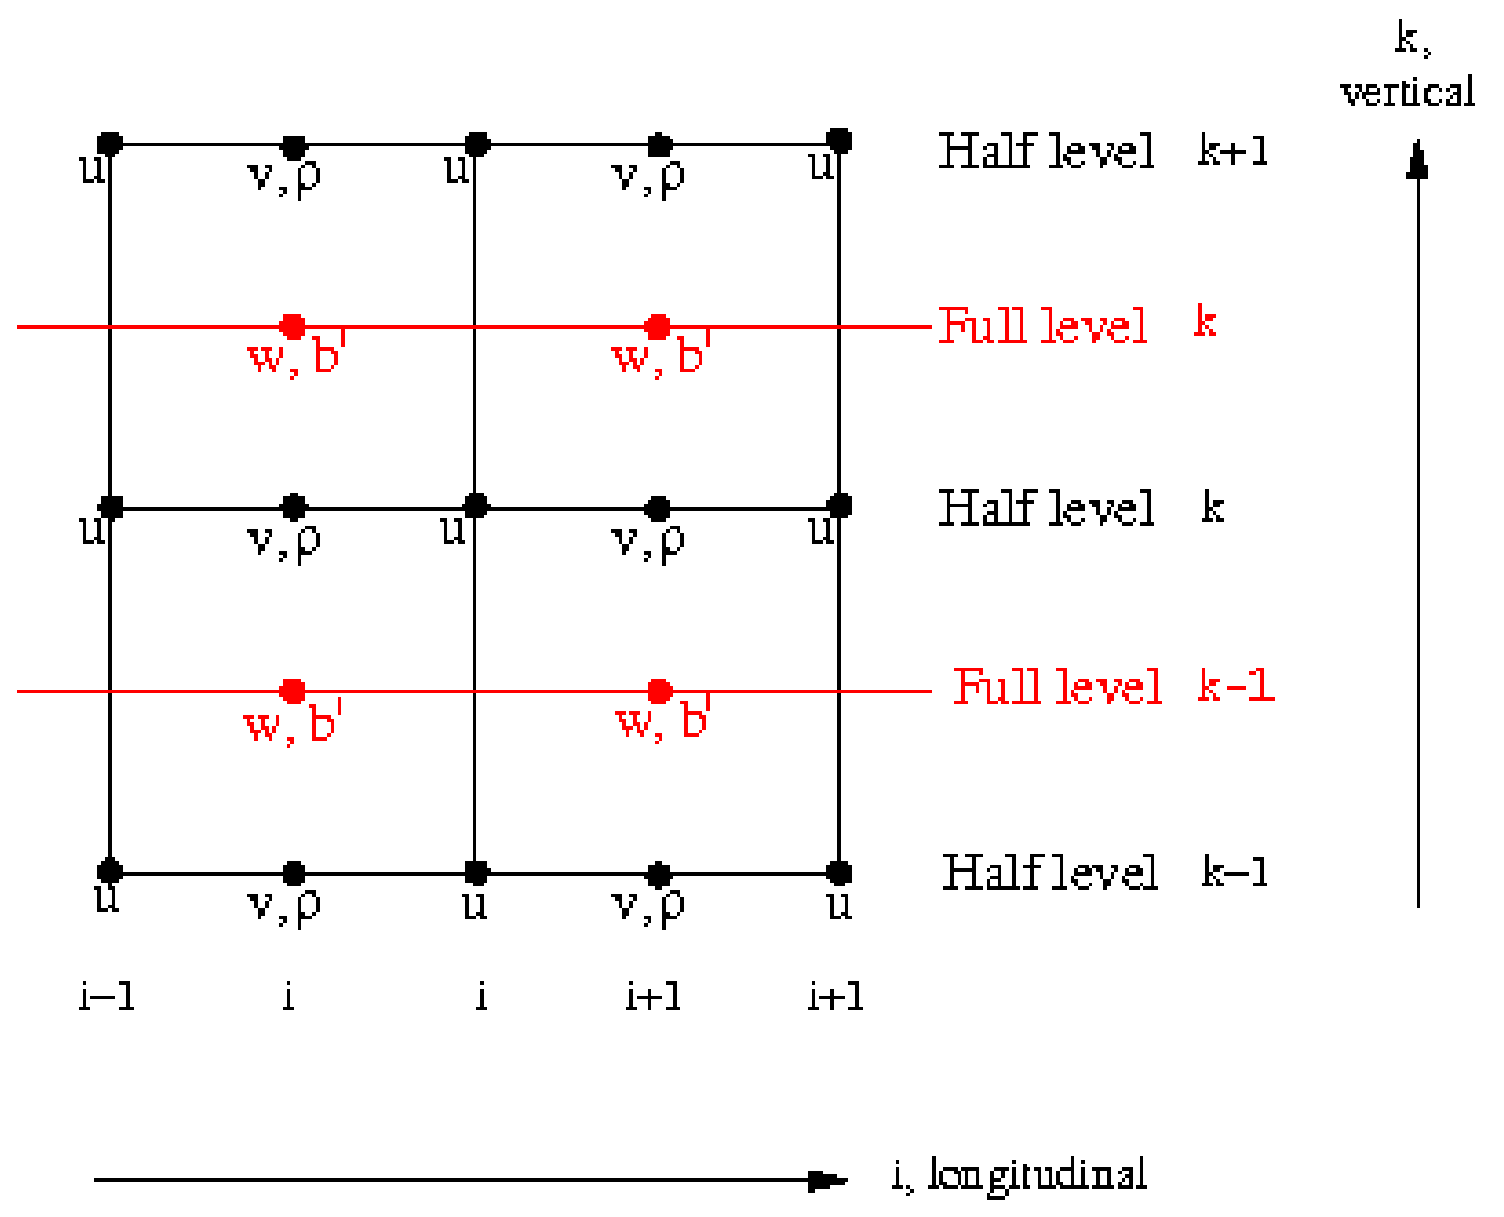
\includegraphics[scale=0.8]{grid1.eps}
  \end{center}
\caption{Illustration of the horizontal and vertical arrangement of the variables on the 
grid.  An Arakawa-C grid is used in the horizontal and a Charney-Phillips grid is used in the vertical}
\label{f_grid}
\end{figure}  
%^^^^^^^^^^^^^^^^^^^^^^^^^^^^^^^^^^^^^^^^^^^^^^^^^^^^^^^^^^^^^^^^^^^^^^^^^^^^^^^^^^^^^^^^^^^^^^^^^^^

This grid facilitates a natural discretization of the equations which does not require significant 
numbers of interpolations.  There are approximately $10^5$ variables in the state space of the toy system.

\subsection{Boundary conditions}

The vertical boundary conditions are summarized in Table \ref{vbcs}.
At the lower boundary the horizontal winds are zero by the no-slip condition and the vertical wind 
is zero to conserve total mass.
At the upper and lower boundaries and the vertical derivative of density is zero.  
The hydrostatic relationship (\ref{hydrostatic_bal}) implies that $b'$ is zero at the boundaries.
At the upper boundary the horizontal winds are chosen to maintain consistency with the boundary 
conditions of $\tilde{p}'$ and $b'$ through thermal wind balance and the vertical wind is again 
zero to conserve total mass.
%
%---------------------------------------------------------------------------------------------------
\begin{table}[ht!]
 \begin{center}
 \setlength{\extrarowheight}{0.2cm}

  \begin{tabular}{|c|c|c|}%{0.5\textwidth}{@{\extracolsep{\fill}} | c | c | c | }
    \hline
           & Lower   & Upper \\ \hline
    $ u $  & $u(z_0) = 0$                                  & $\frac{\partial u(z_t)}{\partial z} = 0 $    \\[1.05ex]\hline
    $ v $  & $v(z_0) = 0$                                  & $\frac{\partial v(z_t)}{\partial z} = 0 $    \\[1.05ex]\hline
    $ w $  & $w(z_0) = 0$                                  & $w(z_t)=0 $      \\[1.05ex] \hline
   $\tilde{p}'$ & $\frac{\partial \tilde{p}'(z_0)}{\partial z} = 0 $ & $\frac{\partial \tilde{p}'(z_t)}{\partial z} = 0 $    \\[1.05ex] \hline
   $ b' $  & $b'(z_0) = 0$                                 & $b'(z_t) = 0$    \\[1.05ex]
    \hline
  \end{tabular}
 \caption{Upper and lower boundary conditions on each prognostic model variable, $z_0$ is the the lower boundary and $z_t$ is the upper boundary. The boundary condition on $b'$ does not need to be explicitly set as it is implied by the hydrostatic relationship
 (\ref{hydrostatic_bal}). }
 \label{vbcs}
 \end{center}
\end{table}
%---------------------------------------------------------------------------------------------------

\subsection{Numerical differentiation and integration}

The spatial derivatives are evaluated using a centred finite difference scheme.
The advective terms are evaluated using a forward upstream scheme (e.g \cite{num_rec}).  
This is a diffusive scheme and more accurate schemes will be considered for future work.  

\subsubsection{Time integration scheme}

The time integration is evaluated using a split explicit, forward-backward scheme \citep{cullen_spex}.  
The forward-backward scheme operates over a time-step $\Delta t$ and comprises two stages, an
adjustment and an advection stage.

\subsubsection*{Adjustment stage}

The adjustment stage operates over a shorter subtime-step $\delta t$, where $\Delta t = n \delta t$ and
$n$ is typically small (in this implementation $n=2$).  
The adjustment stage contains two parts and is iterated $n$ times. 
Let $t_i$ denote a discrete time, and let the notation $t_{i+n}$ be shorthand for $t_{i + n\delta t}$, 
then the following is the general description of the $n^{\rm {th}}$ iteration of the adjustment step. 

The first part of the adjustment stage is the forward part of the forward-backward scheme,
the momentum and thermodynamic equations are evaluated with the advective terms omitted.
% 
The $u$- and $v$-momentum equations are considered simultaneously to find an adjustment due to the 
Coriolis term. Then the $w$-momentum and thermodynamic equations are dealt with simultaneously 
to find the adjustment due to the buoyancy frequency, $A$. 
%
Firstly consider the adjustment due to the Coriolis term. 
The equations for $u$ (\ref{u_final}) and $v$ (\ref{v_final}) with advective terms omitted are
discretized as
%^^^^^^^^^^^^^^^^^^^^^^^^^^^^^^^^^^^^^^^^^^^^^^^^^^^^^^^^^^^^^^^^^^^^^^^^^^^^^^^^^^^^^^^^^^^^^^^^^^^
  \begin{eqnarray}
     u(t_{i+1}) &=& u(t_i) - \delta t \frac{\partial \tilde{p}(t_i)}{\partial x} + 
                 \frac {\delta t f }{2} \left( v(t_i) + v(t_{i+1}) \right),  \label{u_semi}  \\
    v(t_{i+1}) &=& v(t_i) - \frac {\delta t f }{2} \left( u(t_i) + u(t_{i+1}) \right).
    \label{v_semi}
  \end{eqnarray}
%^^^^^^^^^^^^^^^^^^^^^^^^^^^^^^^^^^^^^^^^^^^^^^^^^^^^^^^^^^^^^^^^^^^^^^^^^^^^^^^^^^^^^^^^^^^^^^^^^^^
Solving (\ref{u_semi}) and (\ref{v_semi}) for $u(t_{i+1})$ and $v(t_{i+1})$ gives
%
%^^^^^^^^^^^^^^^^^^^^^^^^^^^^^^^^^^^^^^^^^^^^^^^^^^^^^^^^^^^^^^^^^^^^^^^^^^^^^^^^^^^^^^^^^^^^^^^^^^^
\begin{eqnarray} 
u(t_{i+1}) &=& \frac{\beta_f}{\alpha_f} u(t_i) - \frac {\delta t}{\alpha_f} 
\frac{\partial \tilde{p}(t_i)}{\partial x} + \frac{\delta t f}{\alpha_f} v(t_i), \label{u_semi_5} \\
 v(t_{i+1})&=& \frac{\beta_f}{\alpha_f} v(t_i) - \frac{\delta t f}{\alpha_f} u(t_i) +
 \frac {\delta t^2 f }{2 \alpha_f} \frac{\partial \tilde{p}(t_i)}{\partial x}. 
 \label{v_semi_5}
\end{eqnarray}
%^^^^^^^^^^^^^^^^^^^^^^^^^^^^^^^^^^^^^^^^^^^^^^^^^^^^^^^^^^^^^^^^^^^^^^^^^^^^^^^^^^^^^^^^^^^^^^^^^^^
where $\alpha_f$ and $\beta_f$ are defined by
%^^^^^^^^^^^^^^^^^^^^^^^^^^^^^^^^^^^^^^^^^^^^^^^^^^^^^^^^^^^^^^^^^^^^^^^^^^^^^^^^^^^^^^^^^^^^^^^^^^^
\begin{equation}\label{def_alpha_beta_f}
\alpha_f = \left( 1 + \frac{\delta t^2 f^2}{4} \right), \quad \mbox{and} \quad
\beta_f = \left( 1 - \frac{\delta t^2 f^2}{4} \right).
\end{equation}
%^^^^^^^^^^^^^^^^^^^^^^^^^^^^^^^^^^^^^^^^^^^^^^^^^^^^^^^^^^^^^^^^^^^^^^^^^^^^^^^^^^^^^^^^^^^^^^^^^^^
%
Now consider the adjustment due to the buoyancy frequency term. 
The equations for $w$ (\ref{w_final}) and $b'$ (\ref{thermo_final}) omitting advective terms are 
discretized as
%^^^^^^^^^^^^^^^^^^^^^^^^^^^^^^^^^^^^^^^^^^^^^^^^^^^^^^^^^^^^^^^^^^^^^^^^^^^^^^^^^^^^^^^^^^^^^^^^^^^
\begin{eqnarray} 
w(t_{i+1}) &=& w(t_i) - \delta t \frac{\partial \tilde{p}(t_i)}{\partial z} + 
\frac {\delta t }{2} \left( b'(t_i) + b'(t_{i+1}) \right),\label{w_semi} \\
b'(t_{i+1}) &=& b'(t_i) - \frac {\delta t A^2 }{2} \left( w(t_i) + w(t_{i+1}) \right).
\label{bp_semi}
\end{eqnarray}
%^^^^^^^^^^^^^^^^^^^^^^^^^^^^^^^^^^^^^^^^^^^^^^^^^^^^^^^^^^^^^^^^^^^^^^^^^^^^^^^^^^^^^^^^^^^^^^^^^^^
Solving (\ref{w_semi}) and (\ref{bp_semi}) for $w(t_{i+1})$ and $b'(t_{i+1})$ gives
%^^^^^^^^^^^^^^^^^^^^^^^^^^^^^^^^^^^^^^^^^^^^^^^^^^^^^^^^^^^^^^^^^^^^^^^^^^^^^^^^^^^^^^^^^^^^^^^^^^^
  \begin{eqnarray} 
    w(t_{i+1}) &=& \frac{\beta_A}{\alpha_A} w(t_i) - \frac {\delta t }{\alpha_A} 
    \frac{\partial \tilde{p}(t_i)}{\partial z} + 
      \frac{\delta t }{\alpha_f} b'(t_i), \label{w_semi_5} \\ 
     b'(t_{i+1}) &=& \frac{\beta_A}{\alpha_A} b'(t_i) - \frac{\delta t A^2}{\alpha_A} w(t_i) 
     + \frac {\delta t^2 A^2 }{2 \alpha_A}
     \frac{\partial \tilde{p}(t_i)}{\partial z}.
     \label{bp_semi_4}  
  \end{eqnarray}
%^^^^^^^^^^^^^^^^^^^^^^^^^^^^^^^^^^^^^^^^^^^^^^^^^^^^^^^^^^^^^^^^^^^^^^^^^^^^^^^^^^^^^^^^^^^^^^^^^^^
where $\alpha_A$ and $\beta_A$ are defined by
%^^^^^^^^^^^^^^^^^^^^^^^^^^^^^^^^^^^^^^^^^^^^^^^^^^^^^^^^^^^^^^^^^^^^^^^^^^^^^^^^^^^^^^^^^^^^^^^^^^^
\begin{equation} \label{def_alpha_beta_A}
\alpha_A = \left( 1 + \frac{\delta t^2 A^2}{4} \right), \quad \mbox{and} \quad
\beta_A = \left( 1 - \frac{\delta t^2 A^2}{4} \right).
\end{equation}
%^^^^^^^^^^^^^^^^^^^^^^^^^^^^^^^^^^^^^^^^^^^^^^^^^^^^^^^^^^^^^^^^^^^^^^^^^^^^^^^^^^^^^^^^^^^^^^^^^^^
Equations (\ref{u_semi_5}), (\ref{v_semi_5}), (\ref{w_semi_5}) and (\ref{bp_semi_4}) are 
the discretized forms of the split-explicit equations that are evaluated in the forward part 
of the forward-backward scheme in the adjustment stage. 

The second part of the adjustment stage is the backward part of the forward-backward scheme. 
The continuity equation (\ref{cont_final}) is evaluated using the wind and buoyancy data calculated in
the forward part, i.e.
%^^^^^^^^^^^^^^^^^^^^^^^^^^^^^^^^^^^^^^^^^^^^^^^^^^^^^^^^^^^^^^^^^^^^^^^^^^^^^^^^^^^^^^^^^^^^^^^^^^^
  \begin{equation}
    \tilde{p}'(t_{i+1}) = B \nabla \left(\tilde{p}(t_i) \mathbf u(t +\delta t) \right).
  \end{equation}
%^^^^^^^^^^^^^^^^^^^^^^^^^^^^^^^^^^^^^^^^^^^^^^^^^^^^^^^^^^^^^^^^^^^^^^^^^^^^^^^^^^^^^^^^^^^^^^^^^^^
The adjustment stage is iterated $n$ times. After integration over the full time-step ($\Delta t$) 
the value of $\tilde{p}'$ is known and the values of the variables $u$, $v$, $w$ and $b'$ are known
but their advection has not been included.

\subsubsection*{Advection stage}

The second stage is the advection stage, in this stage the values of the variables $u$, $v$, $w$ and 
$b'$ calculated in the adjustment stage are advected using the average values of the advecting winds. 
The average values of the advecting winds $\bar u$ and $\bar w$ (that are valid over the full 
time-step $\Delta t$) are calculated using data from the adjustment stage.
Let $\phi$ be any of $u$, $v$, $w$ or $b'$ then the advection step is given by
%^^^^^^^^^^^^^^^^^^^^^^^^^^^^^^^^^^^^^^^^^^^^^^^^^^^^^^^^^^^^^^^^^^^^^^^^^^^^^^^^^^^^^^^^^^^^^^^^^^^
  \begin{equation}
    \phi(t + \Delta t) = \phi(t) - \Delta t B \overline {\mathbf u} \cdot \nabla \phi(t),
  \end{equation}
%^^^^^^^^^^^^^^^^^^^^^^^^^^^^^^^^^^^^^^^^^^^^^^^^^^^^^^^^^^^^^^^^^^^^^^^^^^^^^^^^^^^^^^^^^^^^^^^^^^^
where $\overline {\mathbf u}$ is a vector of the average winds. 

\subsubsection*{Overall properties}



The spatial derivatives evaluated by the forward-upstream scheme are first order accurate
\citep{num_rec}. 
The time integration which utilises a split-explicit and forward-backward scheme is first-order
accurate \citep{ames, gadd}. 
The stability of the forward-backward scheme increases the time-steps which are  permitted by the CFL criterion \citep{ames}. The split-explicit scheme has been
used in various implementations of the UK Met Office's NWP model due to its ability to
conserve mass \citep{gadd, cullen_spex}.


%===================================================================================================
\section{Linear analysis}\label{linanal}

In this section a normal mode analysis is performed, this follows the same 
procedure that is demonstrated by for example \cite{daley_1991} and \cite{cullen_book} 
in performing a normal mode analysis of the shallow water equations. 

The linear analysis permits examination of the speeds of the modes present in the model. 
For simplicity this analysis is performed in a triply periodic domain.

%---------------------------------------------------------------------------------------------------
\subsection{Linearisation}
The non-linear model equations (\ref{final_eqns}) are linearized about the reference state and a 
state of rest.    
It is convenient to write the model equations in terms of velocity potential, $\chi$, and 
streamfunction, $\psi$. Where the flow is homogeneous in the meridional direction $\chi$ and $\psi$ 
are defined using Helmholtz theorem:
$u =  {\partial \chi}/{\partial x}$ and $v =   {\partial \psi }/{\partial x}$.
The linearized model equations expressed in terms of velocity potential and divergence are
%
%^^^^^^^^^^^^^^^^^^^^^^^^^^^^^^^^^^^^^^^^^^^^^^^^^^^^^^^^^^^^^^^^^^^^^^^^^^^^^^^^^^^^^^^^^^^^^^^^^^^
\begin{subequations} \label{linear_eqns}
\begin{align} 
\frac{\partial}{\partial t}  \frac{\partial^2 \chi}{\partial x^2} -
 f \frac{\partial^2 \psi}{\partial x^2} + \frac{\partial^2 \tilde{p}'}{\partial x^2} &=0, \label{ucoup}\\
\frac{\partial}{\partial t} \frac{\partial^2 \psi}{\partial x^2} +
 f\frac{\partial^2 \chi}{\partial x^2}  &=0,\label{vcoup} \\
\frac{\partial w}{\partial t} - b' + \frac{\partial \tilde{p}'}{\partial z} &= 0, \label{wcoup}\\
\frac {\partial \tilde{p}'}{\partial t} + B \tilde{p}_0 \frac{\partial^2 \chi}{\partial x^2} +
 B \tilde{p}_0 \frac{\partial w}{\partial z} &= 0, \label{rhocoup}\\
\frac {\partial b'}{\partial t} + A^2w &= 0. \label{bcoup}  
\end{align} 
\end{subequations}
%^^^^^^^^^^^^^^^^^^^^^^^^^^^^^^^^^^^^^^^^^^^^^^^^^^^^^^^^^^^^^^^^^^^^^^^^^^^^^^^^^^^^^^^^^^^^^^^^^^^
%
Now take the following functional dependence for a particular mode:
%^^^^^^^^^^^^^^^^^^^^^^^^^^^^^^^^^^^^^^^^^^^^^^^^^^^^^^^^^^^^^^^^^^^^^^^^^^^^^^^^^^^^^^^^^^^^^^^^^^^
  \begin{eqnarray} \label{eq:fourier}
     \left| \begin{array}{c}
     \chi(x,z,t) \\ \psi(x,z,t) \\ w(x,z,t) \\ \tilde{p}'(x,z,t) \\ b'(x,z,t)  \end{array} \right|  
     &= &\left| \begin{array}{cl} 
     i & \widehat{\chi} \\ & \widehat {\psi} \\  \frac{k}{L_x}  & \widehat{w} \\ \frac {k}{L_x} \sqrt{B \tilde{p}_0}  & \widehat {\tilde{p}'} \\ 
     \frac{-i Ak}   {L_x}  & \widehat{b'} \end{array} \right|  \nonumber \\
     && {\rm{exp}} \left[ i \left\{ \left( \frac{kx}{L_x} \right) + 
     \left( \frac{mz}{L_z} \right) - \sigma f t \right\} \right],
  \end{eqnarray}
%^^^^^^^^^^^^^^^^^^^^^^^^^^^^^^^^^^^^^^^^^^^^^^^^^^^^^^^^^^^^^^^^^^^^^^^^^^^^^^^^^^^^^^^^^^^^^^^^^^^
where $\sigma $ is a dimensionless frequency and $k$ and $m$ are the dimensionless 
horizontal and vertical wave numbers respectively. The domain sizes are given by $L_x$
in the horizontal and $L_z$ in the vertical. 
%
Inserting  (\ref{eq:fourier}) into (\ref{linear_eqns}) and expressing the resultant set
of equations in matrix form gives
%^^^^^^^^^^^^^^^^^^^^^^^^^^^^^^^^^^^^^^^^^^^^^^^^^^^^^^^^^^^^^^^^^^^^^^^^^^^^^^^^^^^^^^^^^^^^^^^^^^^
\begin{equation} \label{eq:spectral_system}
(\mathbf {L} - \sigma \mathbf{I})  
\left| 
  \begin{array}{c} 
       \widehat {\chi} \\ \widehat {\psi} \\  \widehat{w} \\ \widehat {\tilde{p}'} \\ \widehat{b'} 
  \end{array} 
\right| = 0,
\end{equation} 
%^^^^^^^^^^^^^^^^^^^^^^^^^^^^^^^^^^^^^^^^^^^^^^^^^^^^^^^^^^^^^^^^^^^^^^^^^^^^^^^^^^^^^^^^^^^^^^^^^^^
where
%^^^^^^^^^^^^^^^^^^^^^^^^^^^^^^^^^^^^^^^^^^^^^^^^^^^^^^^^^^^^^^^^^^^^^^^^^^^^^^^^^^^^^^^^^^^^^^^^^^^
\begin{equation} \label{eq:def_L_mat}
\mathbf{L} = \left( \begin{array}{c c c c c} 
0 & 1 & 0 & - \frac{k \sqrt{B\tilde{p}_0}}{f L_x} & 0 \\
1 & 0 & 0 & 0 & 0 \\
0 & 0 & 0 & \frac{m \sqrt{B\tilde{p}_0}}{f L_z}& \frac{A}{f}\\
- \frac{k \sqrt{B\tilde{p}_0}}{f L_x} & 0 & \frac{m \sqrt{B\tilde{p}_0}}{f L_z} & 0 & 0 \\
0 & 0 & \frac{A}{f} & 0 &  0  \\
\end{array} \right) 
\end{equation}
%^^^^^^^^^^^^^^^^^^^^^^^^^^^^^^^^^^^^^^^^^^^^^^^^^^^^^^^^^^^^^^^^^^^^^^^^^^^^^^^^^^^^^^^^^^^^^^^^^^^

 
The factors that normalize the terms in  (\ref{eq:fourier}) were chosen such 
that $\mathbf L$ is a real and symmetric matrix.  The determinant of the matrix 
$(\mathbf {L} - \sigma \mathbf{I})$ has to be zero to allow non-trivial solutions 
and so sigma must necessarily be an eigenvalue of $\mathbf L$.
For each distinct pair of horizontal and vertical wavenumbers $(k,m)$, $\mathbf L$ 
has five eigenvectors and eigenvalues.
The five distinct eigenvalues are denoted $\sigma_r$, $\pm \sigma_g$ and $\pm \sigma_a$ where
%^^^^^^^^^^^^^^^^^^^^^^^^^^^^^^^^^^^^^^^^^^^^^^^^^^^^^^^^^^^^^^^^^^^^^^^^^^^^^^^^^^^^^^^^^^^^^^^^^^^
\begin{eqnarray}
\sigma_r &=& 0, \nonumber \\
\sigma_g &=& - \sigma_{g'}, \nonumber \\
\sigma_a &=& - \sigma_{a'}.
\end{eqnarray}
%^^^^^^^^^^^^^^^^^^^^^^^^^^^^^^^^^^^^^^^^^^^^^^^^^^^^^^^^^^^^^^^^^^^^^^^^^^^^^^^^^^^^^^^^^^^^^^^^^^^
These are the three distinct modes that are present in the system, where the subscripts $r$ represent a Rossby-like mode, $g$ and $g'$ inertia gravity modes, and $a$ and $a'$ acoustic modes. 
We can see from (\ref{eq:def_L_mat}) that the terms in the top left block of ${\mathbf L}$ represent inertial oscillations with dimensional frequency $f$. The terms in the fourth row and fourth column represent acoustic waves with dimensional speed of sound $\sqrt{B \tilde {p_0} }$. 
The remaining terms represent buoyancy oscillations with dimensional frequency $A$.




The algebraic forms of the eigenvectors of the gravity and acoustic modes are very complicated (these
modes are only considered further numerically).
The algebraic form of the Rossby-like mode is simple and is now considered in more detail.


%---------------------------------------------------------------------------------------------------
\subsection{The Rossby-like mode}

The unit eigenvector corresponding to the eigenvalue $ \sigma_r = 0$ is 
%^^^^^^^^^^^^^^^^^^^^^^^^^^^^^^^^^^^^^^^^^^^^^^^^^^^^^^^^^^^^^^^^^^^^^^^^^^^^^^^^^^^^^^^^^^^^^^^^^^^
 \begin{equation} \label{rossby_eig}
   \left ( 
     \begin{array}{c} 
       \widehat \chi \\ \widehat \psi \\ \widehat w \\ \widehat {\tilde{p}'} \\ \widehat b' 
     \end{array} 
   \right) 
   = \frac 1{\sqrt{K}}
      \left ( 
       \begin{array}{c} 
         0 \\ -\frac{kAL_z}{L_xfm} \\ 0 \\ -\frac{AL_z}{ m \sqrt{B\tilde{p}_0}} \\ 1 
       \end{array} 
      \right),
 \end{equation} 
%^^^^^^^^^^^^^^^^^^^^^^^^^^^^^^^^^^^^^^^^^^^^^^^^^^^^^^^^^^^^^^^^^^^^^^^^^^^^^^^^^^^^^^^^^^^^^^^^^^^
where $K$ is the normalization factor $K = (A L_z[k B\tilde{p}_0 + L_x f^2] + L_x^2 f^2 m^2 B\tilde{p}_0)/(L_x^2 f^2 m^2 B\tilde{p}_0)$.

It can be shown that this mode supports geostrophic flow. 
The geostrophic relationships for the model equations (defined in section \ref{sec:scale_anal} 
but repeated here for convenience) are
%^^^^^^^^^^^^^^^^^^^^^^^^^^^^^^^^^^^^^^^^^^^^^^^^^^^^^^^^^^^^^^^^^^^^^^^^^^^^^^^^^^^^^^^^^^^^^^^^^^^
  \begin{eqnarray}
    \frac {\partial \tilde{p}' }{\partial x} &=& f v, \label{geost} \quad \mbox{and} \\
    \quad u &=& 0. \label{geost2}
  \end{eqnarray}
%^^^^^^^^^^^^^^^^^^^^^^^^^^^^^^^^^^^^^^^^^^^^^^^^^^^^^^^^^^^^^^^^^^^^^^^^^^^^^^^^^^^^^^^^^^^^^^^^^^^
The second geostrophic relation  (\ref{geost2}) is easily satisfied for the first 
eigenvalue $\sigma_r =0$.  Since the second equation from (\ref{eq:spectral_system}) gives 
$\widehat \chi = 0$  and $ \left (u = {\partial \chi}/{\partial x} \right )$ it immediately 
follows that $u = 0$.   
The first and non-trivial geostrophic shiprelation (\ref{geost}) when
written in spectral space using (\ref{eq:fourier}) for a given wavenumber $k$ is 
%^^^^^^^^^^^^^^^^^^^^^^^^^^^^^^^^^^^^^^^^^^^^^^^^^^^^^^^^^^^^^^^^^^^^^^^^^^^^^^^^^^^^^^^^^^^^^^^^^^^
   \begin{equation}  \label{psuedo_geost} 
      \frac{k}{L_x} \sqrt{B\tilde{p}_0} \widehat {\tilde{p}'} = f \widehat \psi.
   \end{equation}
%^^^^^^^^^^^^^^^^^^^^^^^^^^^^^^^^^^^^^^^^^^^^^^^^^^^^^^^^^^^^^^^^^^^^^^^^^^^^^^^^^^^^^^^^^^^^^^^^^^^
%
Substituting the $\widehat{\psi}$ and $\widehat{\tilde p}'$ components of (\ref{rossby_eig}) into 
(\ref{psuedo_geost}) demonstrates that the first eigenmode supports geostrophic motion. 
It is termed Rossby-like since there is an additional component pertaining to $b'$

It can also be shown that this mode supports hydrostatic flow.
The hydrostatic relationship (\ref{hydrostatic_bal}) also repeated here for convenience is
%^^^^^^^^^^^^^^^^^^^^^^^^^^^^^^^^^^^^^^^^^^^^^^^^^^^^^^^^^^^^^^^^^^^^^^^^^^^^^^^^^^^^^^^^^^^^^^^^^^^
  \begin{equation}
    \frac {\partial \tilde{p}'}{\partial z} = b', \label{e_hyrdo_bal_rossby}
  \end{equation}
%^^^^^^^^^^^^^^^^^^^^^^^^^^^^^^^^^^^^^^^^^^^^^^^^^^^^^^^^^^^^^^^^^^^^^^^^^^^^^^^^^^^^^^^^^^^^^^^^^^^
Written in spectral space using (\ref{eq:fourier}) the hydrostatic balance relationship becomes
%^^^^^^^^^^^^^^^^^^^^^^^^^^^^^^^^^^^^^^^^^^^^^^^^^^^^^^^^^^^^^^^^^^^^^^^^^^^^^^^^^^^^^^^^^^^^^^^^^^^
 \begin{equation} \label{e_psuedo_hydro} 
   i \frac {k m \sqrt{BP_0}} {L_x L_z} \widehat{\tilde{p}'} = -i \frac{Ak}{L_x} \widehat {b}' .
 \end{equation}
%^^^^^^^^^^^^^^^^^^^^^^^^^^^^^^^^^^^^^^^^^^^^^^^^^^^^^^^^^^^^^^^^^^^^^^^^^^^^^^^^^^^^^^^^^^^^^^^^^^^
Substituting the $\widehat{p}'$ and $\widehat{b}'$ components of (\ref{rossby_eig}) into 
(\ref{e_psuedo_hydro}) demonstrates that the first eigenmode supports hydrostatic flow 
(with an additional component pertaining to $\widehat \psi$).  


%---------------------------------------------------------------------------------------------------


%%%%%%%%%%%%%%%%%%
% TO BE INCLUDED IN RESULTS AND DISCUSSION SECTION
%%%%%%%%%%%%%%%%%%%
% Since (\ref{simp_eqnstate}) is used in the momentum equations (although since the model is 
%homogeneous in the meridional there is no meridional pressure gradient term) then the chosen value 
%of $C$ has a physical impact on the system.  An estimate of the value of $C$ can be estimated 
%from some sample data. Values of $C$ that are greater than the estimated value increase the 
%strength of the pressure gradients in the system and conversely values of $C$ that are smaller 
%than the estimated value decrease the strength of the pressure gradients.


\begin{thebibliography}
%\bibliographystyle{wileyqj}

\bibitem[Ames (1969)]{ames}
Ames~W.F. 1969. Numerical methods for partial differential equations.
\emph{London, Nelson};   

\bibitem[Bannister(2008)]{bannister_2008_2}
Bannister~R.N. A review of forecast error covariance statistics in atmospheric variational data assimilation. II: Modelling the forecast error covariance statistics.
\emph{Q. J. R. Meteorol. Soc.}; 134:1971-1996

\bibitem[Baxter et al(2010)]{baxter}
Baxter~G.M., Dance~S.L., Lawless~A.S., Nichols~N.K. 2010. Four-dimensional variational data
assimilation for high resolution nested models. 
\emph{Comput. Fluids}; 46:137-141

\bibitem[Bryan et al(2003)]{bryan_2003}
Bryan~G.H., Wyngaard~J.C., Fritsch~J.M. 2003. Resolution requirements for the
simulation of deep moist convection.
\emph{Mon. Wea. Rev.}; 131:2394–2416.

\bibitem[Clark et al(2003)]{clark_2005}
Clark~P.A., Browning~K.A.,  Wang~C. 2005. The sting at the end of the tail: Model diagnostics of fine-scale
three-dimensional structure of the cloud head.
\emph{Q. J. R. Meteorol. Soc.}; 131:2263–2292

\bibitem[Cullen (2006)]{cullen_book}
Cullen~M.J.P. 2006. A mathematical theory of large-scale atmosphere/ocean flow.
\emph{Imperial College Press};   
 
\bibitem[Cullen and Davies(1991)]{cullen_spex}
Cullen~M.J.P., Davies~T. 1991. A conservative split-explicit integration scheme with fourth-order horizontal advection.
\emph{Q. J. R. Meteorol. Soc.}; 117:993-1002

\bibitem[Daley(1991)]{daley_1991}
Daley~R. 1991. Atmospheric data analysis.
\emph{Cambridge University Press.}

\bibitem[Dance(2004)]{dance_2004}
Dance~S.L. 2004. Issues in high resolution limited area data assimilation for quantitative
precipitation forecasting. 
\emph{Physica D}; 196:1–27.

\bibitem[Davies et al(2005)]{davies_2005}
Davies~T., Cullen~M.J.P., Malcolm~A.J., Mawson~A.S.M.H., White~A.A., Wood~N. 2005. A new dynamical core for the Met Office's global and regional modelling of the atmosphere.
\emph{Q. J. R. Meterol. Soc.}; 131:1759-1782.

\bibitem[Dixon et al(2009)]{dixon_2009}
Dixon~M., Zhihong~L., Lean~H., Roberts~N., Ballard~S.P. 2009. Impact of data assimilation on forecasting convection over the United Kingdom using a high resolution version of the Met Office Unified Model.
\emph{Mon. Wea. Rev.}; 137:1562-1584.

\bibitem[Gadd (1978)]{gadd}
Gadd~A.J. 1978. A split explicit integration scheme for numerical weather prediction.
\emph{Q. J. R. Meterol. Soc.}; 104:569-582.

\bibitem[Gill(1982)]{gill}
Gill~A.E. 2004. Atmosphere-Ocean Dynamics. 
\emph{Academic Press.} 

\bibitem[Holton(2004)]{holton}
Holton~J.R. 2004. An Introduction to Dynamic Meteorology, 4 edition. 
\emph{Academic Press.} 

\bibitem[Kalnay(2002)]{kalnay}
Kalnay~E. 2002. Atmospheric modeling, data assimilation and predictability.
\emph{Cambridge University Press.}

\bibitem[Lean et al(2008)]{lean_2008}
Lean~H., Clark~P.A., Dixon~M., Roberts~N., Fritch~A., Forbes~R., Halliwell~C. 2008. Characteristics of high resolution versions of the Met Office Unified Model for forecasting convection over the United Kingdom.
\emph{Mon. Wea. Rev.}; 136:3408-3424.

\bibitem[Lorenc et al(2000)]{lorenc_2000}
Lorenc~A.C., Ballard~S.P., Bell~R.S., Ingelby~N.B., Andrews~P.L.F., Barker~D.M., Bray~J.R., Clayton~A.M., Dalby~T., Li~D., Payne~T.J., Saunders~F.W. 2000. The Met. Office global three-dimensional variational data assimilation scheme. 
\emph{Q. J. R. Meteorol. Soc.}; 126:2991-3012.

\bibitem[Lorenc and Payne(2007)]{lorenc_2007}
Lorenc~A.C., Payne~T. 2007. 4D-Var and the butterfly effect: Statistical fourdimensional
data assimilation for a wide range of scales. 
\emph{Q. J. R. Meteorol. Soc.}; 133:607–614.

\bibitem[Lorenz (1963)]{lorenz}
Lorenz~E.N. 1963. Deterministic non-periodic flow.
\emph{J. Atmos. Sci.}; 20:130-147.


\bibitem[Park and Zupanski(2003)]{park_2003}
Park~S.K., Zupanski~D. 2003. Four-dimensional variational data assimilation for
mesoscale and storm-scale applications. 
\emph{Meteorology and Atmospheric Physics}; 82:173–208.

\bibitem[Pielke(2002)]{pielke}
Pielke~R.A. Sr. Mesoscale Meteorological Modeling.
\emph{Academic Press.}

\bibitem[Press(2007)]{num_rec}
Press~W.H., Teukolsky~S.A., Vetterling~W.T., Flannery~B.P. (2007). Numerical Recipes 3rd Edition: The Art of Scientific Computing.
\emph{Cambridge University Press}

\bibitem[Sun(2005)]{sun_2005}
Sun~J. 2005. Convective-scale assimilation of radar data: Progress and challenges. 
\emph{Q. J. R. Meteorol. Soc.;  131:3439–3463.}

\bibitem[Thuburn et al (2002)]{thuburn1}
Thuburn~J., Wood~N., Staniforth~A. 2002. Normal modes of deep atmospheres I: Spherical geometry
\emph{Q. J. R. Meteorol. Soc.; 128:1771-1792.}

%\bibitem[Thuburn et al (2002)]{thuburn2}
%Thuburn~J., Wood~N., Staniforth~A. 2002. Normal modes of deep atmospheres II: f-F-plane geometry
%\emph{Q. J. R. Meteorol. Soc.; 128:1793-1806.}

\bibitem[Vallis(2006)]{vallis}
Vallis~G.K. 2006. Atmospheric and oceanic fluid dynamics.
\emph{Cambridge University Press.}

\bibitem[Vetra-Carvalho et al(2010)]{vetra_2012}
Vetra-Carvalho~S., Dixon~M., Migliorini~S., Nichols~N.K., Ballard~S.P. 2010. Breakdown of hydrostatic balance at convective-scales in forecast errors in the Met Office Unified Model.
Submitted to \emph{Q. J. R. Meterol. Soc.}

\end{thebibliography}
\end{document}

